\documentclass[12pt,a4paper]{article}
%-- coding: UTF-8 --
\usepackage[UTF8]{ctex}
\usepackage[utf8]{inputenc}
\usepackage{geometry}
\usepackage{graphicx} % 引入图片
\usepackage{enumitem} % 取消列表默认间距
\geometry{left=3.18cm,right=3.18cm,top=2.54cm,bottom=2.54cm}
\usepackage{hyperref}
\hypersetup{hidelinks,
	colorlinks=true,
	allcolors=black,
	pdfstartview=Fit,
	breaklinks=true}
\usepackage{listings}
\usepackage{xcolor}
\usepackage{fontspec}
\usepackage{booktabs} % 三线表
\usepackage{float}

\usepackage{tikz}
\usepackage{amsmath}
\usepackage{colortbl}
\newcommand\y{\cellcolor{clight2}}
\definecolor{clight2}{RGB}{212, 237, 244}%
\newcommand\tikznode[3][]%
   {\tikz[remember picture,baseline=(#2.base)]
      \node[minimum size=0pt,inner sep=0pt,#1](#2){#3};%
   }
\tikzset{>=stealth}
\renewcommand\vec[1]{\mathbf{#1}}

% 嵌入代码风格
\lstset{
	language    = c++,
	breaklines  = true,
	captionpos  = b,
	tabsize     = 4,
	columns     = fullflexible,
	commentstyle = \color[RGB]{0,128,0},
	keywordstyle = \color[RGB]{0,0,255},
	basicstyle   = \small\ttfamily,
	stringstyle  = \color[RGB]{148,0,209}\ttfamily,
	rulesepcolor = \color{red!20!green!20!blue!20},
	showstringspaces = false,
}


%伪代码
\usepackage{multirow}
\usepackage{algorithm}
\usepackage[noend]{algpseudocode}
\usepackage{amsmath}

\title{实验三 \hspace{0.5cm} 堆排序与快速排序}
\author{
\begin{tabular}{c @{\hspace{5mm}} c}
    黄韦杰 & 刘嘉杰 \\  % 作者名
    \href{mailto:hwj@hust.edu.cn}{hwj@hust.edu.cn} & \href{mailto:m202474039@hust.edu.cn}{m202474039@hust.edu.cn} % 邮箱
\end{tabular}
}
\date{October, 2024}

\begin{document}
\maketitle

\section{前言}

\subsection{堆排序}

堆排序是基于二叉堆而实现的排序,它可以在 $O(\log n)$ 的时间内插入、删除元素,并 $O(1)$ 地返回当前集合的最大值或最小值,借助选择排序的思想,堆排序可以在 $O(n\log n)$ 的时间内完成数组的排序。

二叉堆是一个完全二叉树,当树中任意一个节点的权值都大于等于它儿子的权值,那么它是一个大根堆,当树中任意一个节点的权值都小于等于它儿子的权值,那么它是一个小根堆。

\begin{figure}[H]
    \centering
    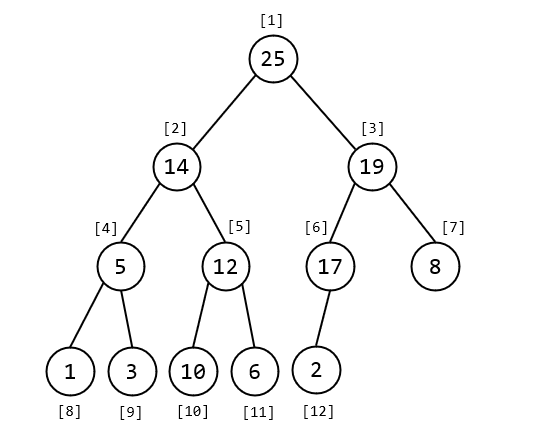
\includegraphics[width=8cm]{img/lab3/heap.png}
    \caption{大根堆}
    \label{fig:my_label}
\end{figure}

以下标为 1 开始的数组 heap:[25,14,19,5,12,17,8,1,3,10,6,2] 表示的二叉堆如图 1 所示。容易发现,节点 $x$ 的左孩子为 $2x$,右孩子为 $2 x + 1$,父亲节点为 $\lfloor x/2\rfloor$。因此,我们可以很容易地用根结点下标为 1 的数组来表示一个二叉堆。

更进一步的,长度为 $n$ 的数组若要表示为一个完全二叉树,只有下标范围在 $[1, n/2]$ 中的元素才会作为非叶子节点。基于这一性质,我们可以直接从 $\lfloor n / 2 \rfloor$ 倒序建堆,当建立以 $i$ 节点为根的二叉堆时,我们假定它的两个子树:以 $2i$ 和 $2i+1$ 为根结点的子树都已经是二叉堆。构建的伪代码如下:

\begin{algorithm}[h]
    \caption{Max-Heapify}
    \begin{algorithmic}[1]
        \Require
        the binary trees rooted at 2i and 2i+1 are submaxheaps
        \Function{Max-Heapify}{$A, i$}
        \State $l = 2\times i$
        \State $r = 2\times i+1$
        \If{ $l \le A.heapsize$ and $A[l] > A[i]$}
        \State $largest = l$
        \Else
        \State $largest = i$
        \EndIf
        \If{ $r \le A.heapsize$ and $A[r] > A[largest]$ }
        \State $largest = r$
        \EndIf
        \If{$largest \neq i$}
        \State $swap(A[i], A[largest])$
        \State \Call{max-heapify}{$A, largest$}
        \EndIf
        \EndFunction
    \end{algorithmic}
\end{algorithm}

由此,我们以 Down-To-Top 的顺序建立二叉堆:
\begin{algorithm}[h]
    \caption{Build-Max-Heap}
    \begin{algorithmic}[1]
        \Function{Build-Max-Heap}{$A$}
        \State $A.heapsize = A.length$
        \For{ i = $\lfloor A.length / 2 \rfloor$ \textbf{downto} 1}
        \State \Call{max-heapify}{$A, i$}
        \EndFor
        \EndFunction
    \end{algorithmic}
\end{algorithm}

由于堆顶元素为堆中最大值,所以我们依旧按照 Down-To-Top 的顺序对数组进行排序:

\begin{algorithm}[h]
    \caption{HEAPSORT}
    \begin{algorithmic}[1]
        \Function{HEAPSORT}{$A$}
        \State \Call{BUILD-MAX-HEAP}{A}
        \For{ $i = A.length$ \textbf{downto} 2}
        \State $swap(A[1], A[i])$
        \State $A.heapsize = A.heapsize - 1$
        \State \Call{MAX-HEAPIFY}{$A, 1$}
        \EndFor
        \EndFunction
    \end{algorithmic}
\end{algorithm}

看起来建堆的复杂度为 $O(n\log n)$,实则不然。假设树高 $h = \log n$,第 $h$ 层为叶子结点,在对第 $x$ 层的节点 $i$ 调整时,\text{MAX-HEAPIFY} 最多会调用 $h - x$ 次,而第 $x$ 层的结点数最多有 $2^{x-1}$ 个。所以总调用次数为:$\sum_{x = 1}^{h} 2^{x-1} (h-x)$。该式是一个等比数列,可以用错位相减法求渐近复杂度,化简可得 $O(n)$。

\subsection{快速排序}

快速排序(Quicksort),又称分区交换排序(partition-exchange sort),简称快排,是一种被广泛运用的排序算法。它的原理是分治算法,主要过程如下:

\begin{enumerate}[noitemsep]
    \item 将数列划分为两部分(左侧所有元素都小于等于右侧);
    \item 递归两个子序列分别进行快速排序;
    \item 不用合并,因为此时数列已经完全有序。
\end{enumerate}

关键的问题是如何在线性时间内将数组划分为具有相对大小关系的两部分(左边小于等于右边)。为了保证平均复杂度,一般是在原数组中随机选择一个数作为 pivot,通过维护一前一后两个指针 $i$ 和 $j$ 来实现数组的划分操作:

\begin{algorithm}[h]
    \caption{Quick Sort}
    \begin{algorithmic}[1]
        \Function{Partition}{$A, p, q$}
        \State $swap(A[p], A[rand(p, q)])$ \Comment{Randomly choose a number in the range p to q and move it to the first place}
        \State $pivot = A[p]$
        \State $i = p$
        \For{$j = p + 1$ to $q$}
        \If{$A[j] < pivot$}
        \State $i = i + 1$
        \State $swap(A[i], A[j])$
        \EndIf
        \EndFor
        \State $swap(A[i], A[p])$
        \State \Return $i$
        \EndFunction
        \Function{Quick-Sort}{$A, l, r$}
        \If{$l < r$}
        \State $m = $ \Call{Partition}{$A, l, r$}
        \State \Call{quick-sort}{$A, l, m - 1$}
        \State \Call{quick-sort}{$A, m + 1, r$}
        \EndIf

        \EndFunction

        \State QUICK-SORT(A, 1, n) \Comment{Initial call}
    \end{algorithmic}
\end{algorithm}

其实,快速排序没有指定应如何具体实现划分,不论是选择 pivot 的过程还是划分的过程,都有不止一种实现方法。

本节实验的目标是实现堆排序与快速排序。


\newpage

\section{实验项目结构}

\begin{itemize}[noitemsep]
    \item[$-$] include
        \begin{itemize}[noitemsep]
            \item[$\bullet$] util.hpp \textit{常用函数头文件}
            \item[$\bullet$] MySort.hpp \textit{基类 MySort}
            \item[$\bullet$] InsertionSort.hpp \textit{插入排序}
            \item[$\bullet$] MergeSort.hpp \textit{归并排序}
            \item[$\bullet$] HeapSort.hpp \textit{堆排序}
            \item[$\bullet$] QuickSort.hpp \textit{快速排序}
            \item[$\bullet$] ThreeWayQuickSort.hpp \textit{三路快速排序(拓展题)}
        \end{itemize}
    \item[$-$] data
        \begin{itemize}[noitemsep]
            \item[$-$] sample
            \item[$-$] test
            \item[$-$] generate
        \end{itemize}
    \item[$-$] performance
        \begin{itemize}[noitemsep]
            \item[$\bullet$] performance.cpp \textit{性能测试程序代码}
        \end{itemize}
    \item[$\bullet$] main.cpp \textit{主程序代码}
\end{itemize}

本实验代码结构与实验一类似。

\textcolor{red}{请注意,每次修改完代码之后,需要重新编译运行 main.cpp,如果直接执行上次编译好的 main.exe 或 main,新的修改将不会生效。在本地测试通过后请将代码提交到OJ上。}

\section{实验内容}

\subsection{堆排序}

基于前言中介绍的堆排序思想,实现 HeapSort.hpp 中的堆排序函数。

\begin{lstlisting}
    class HeapSort: public MySort {
    public:
        int heap_size;
        int length;
        void max_heapify(std::vector<int>& nums, int i) {
            // 请在这里完成你的代码
        }
        void build_max_heap(std::vector<int>& nums) {
            // 请在这里完成你的代码
        }
        void mysort(std::vector<int>& nums) {
            length = nums.size();
            nums.insert(nums.begin(), 0); // 在开头插入一个元素,使得待排序元素下标从 1 开始
            
            // 请在这里完成你的代码
            
            nums.erase(nums.begin()); // 删除开头元素
        }
    };
\end{lstlisting}



\subsection{快速排序}

基于前言中介绍的快速排序思想,实现 QuickSort.hpp 中的快速排序函数。

\begin{lstlisting}
    class QuickSort: public MySort {
    public:
        int partition(std::vector<int>& nums, int p, int q) {
            // 请在这里完成你的代码
        }
        void quick_sort(std::vector<int>& nums, int l, int r) {
            // 请在这里完成你的代码
        }
        void mysort(std::vector<int>& nums) {
            if(nums.size() == 0) return;
            quick_sort(nums, 0, nums.size() - 1);
        }
    };
\end{lstlisting}




\section{实验思考}

\begin{enumerate}
    \item 以第一组测试数据(直接打断点即可观察)为例,分别观察堆排序和快速排序过程中数组元素的变化情况(需要在报告中给出每一步数组的情况)。
          \begin{itemize}
              \item input \\ 5 \\ 1 6 2 10 2
              \item output \\ 1 2 2 6 10
          \end{itemize}

    \item 比较插入排序、归并排序、堆排序与快速排序的性能差距(通过编译运行 performance.cpp 来对比)。
\end{enumerate}

\section{拓展实验}

\subsection{三路快速排序}

如果数组原本就是升序或者降序的,那么基于随机选择 pivot 的快速排序算法要比朴素的快速排序算法快很多。但如果数组中存在着大量的重复数据,基于随机选择 pivot 的快速排序算法最差复杂度仍旧会变成 $O(n^2)$ 的。一种叫做\textbf{三路快速排序}的优化方法可以解决这个问题,与原始的快速排序不同,三路快速排序在随机选取分界点 pivot 后,将待排数列划分为三个部分:小于 pivot、等于 pivot 以及大于 pivot 。这样做即实现了将与分界元素相等的元素聚集在分界元素周围这一效果。Algorithm 5 展示了三路快速排序的伪代码。
\begin{algorithm}[h]
    \caption{Three-Way-Quick-Sort}
    \begin{algorithmic}[1]
        \Function{THREE-WAY-QUICK-SORT}{$A, p, q$}
        \If{$p >= q$}
        \State \Return
        \EndIf
        \State $pivot = A[rand(p, q)]$
        \State $i = p$ \Comment{\text{$i$ 指向当前要处理的元素}}
        \State $j = p$ \Comment{\text{排序过程中,$[p, j - 1]$ 表示小于 pivot 的区间}}
        \State $k = q$ \Comment{\text{排序过程中,$[k + 1, q]$ 表示大于 pivot 的区间}}
        \While{$i <= k$}
        \If{$A[i] < pivot$}
        \State $swap(A[i], A[j])$
        \State $i = i + 1$
        \State $j = j + 1$
        \ElsIf {$A[i] > pivot$}
        \State $swap(A[i], A[k])$
        \State $k = k - 1$
        \Else
        \State $i = i + 1$
        \EndIf
        \EndWhile
        \State \Call{THREE-WAY-QUICK-SORT}{$A, p, j - 1$}
        \State \Call{THREE-WAY-QUICK-SORT}{$A, k + 1, q$}
        \EndFunction
    \end{algorithmic}
\end{algorithm}

三路快速排序在处理含有多个重复值的数组时,效率远高于原始快速排序。其最佳时间复杂度为 $O(n)$。

\subsection{内省排序}
内省排序(Introsort 或 Introspective sort)是快速排序和 堆排序 的结合,由 David Musser 于 1997 年发明。内省排序其实是对快速排序的一种优化,保证了最差时间复杂度为 $O(n\log n)$。


内省排序将快速排序的最大递归深度限制为 $\lfloor \log n \rfloor$ ,超过限制时就转换为堆排序。这样既保留了快速排序内存访问的局部性,又可以防止快速排序在某些情况下性能退化为 $O(n^2)$。

从 2000 年 6 月起,C++ STL 中的 sort() 函数的实现采用了内省排序算法, 在此实现中,当数据数量少于 16 时,将采用插入排序。Algorithm 6 展示了内省排序的伪代码。


\begin{algorithm}[h]
    \caption{Introsort}
    \begin{algorithmic}[1]
        \Function{sort}{A}
        \State maxdepth = $\lfloor \log_2^{length(A)} \rfloor \times 2$
        \State\Call{introsort}{$A, maxdepth$}
        \EndFunction
        \Function{introsort}{A, maxdepth}
        \State $n = length(A)$
        \If{$n < 16$}
        \State\Call{insertionsort}{A}
        \ElsIf{$maxdepth == 0$}
        \State \Call{heapsort}{A}
        \Else
        \State p = \Call{partition}{A}
        \State \Call{introsort}{$A[1:p-1], maxdepth - 1$}
        \State \Call{introsort}{$A[p + 1:n], maxdepth - 1$}
        \EndIf
        \EndFunction
    \end{algorithmic}
\end{algorithm}

拓展实验仅要求根据上述三路快速排序的伪代码完成 ThreeWayQuickSort.hpp 的实现。

\begin{lstlisting}
class ThreeWayQuickSort: public MySort {
public:
    void three_way_quick_sort(std::vector<int>& nums, int p, int q) {
        // 请在这里完成你的代码
    }
    void mysort(std::vector<int>& nums) {
        if(nums.size() == 0) return;
        three_way_quick_sort(nums, 0, nums.size() - 1);
    }
};
\end{lstlisting}

\section*{更新历史}

\begin{center}
    \begin{tabular}{|c|c|c|}
        \hline
        \textbf{更新时间} & \textbf{助教} & \textbf{更新内容} \\
        \hline
        2024 & 黄韦杰, 刘嘉杰 & 修正建堆表述\\
        2023 & 王梓健, 黄韦杰 & 添加 OJ 相关表述 \\
        2022 & 邢广杰, 李晓晓 & 完善实验题目,开始更新记录 \\
        2021 & 韩耀东 & 主要内容构建 \\
        % Add more rows as needed
        \hline
        \end{tabular}
\end{center}


\end{document}